\chapter{SRIM Results}



\FloatBarrier
\subsection{Ion paths through an iron sample}


\begin{figure}[!htb]
  \begin{center}
    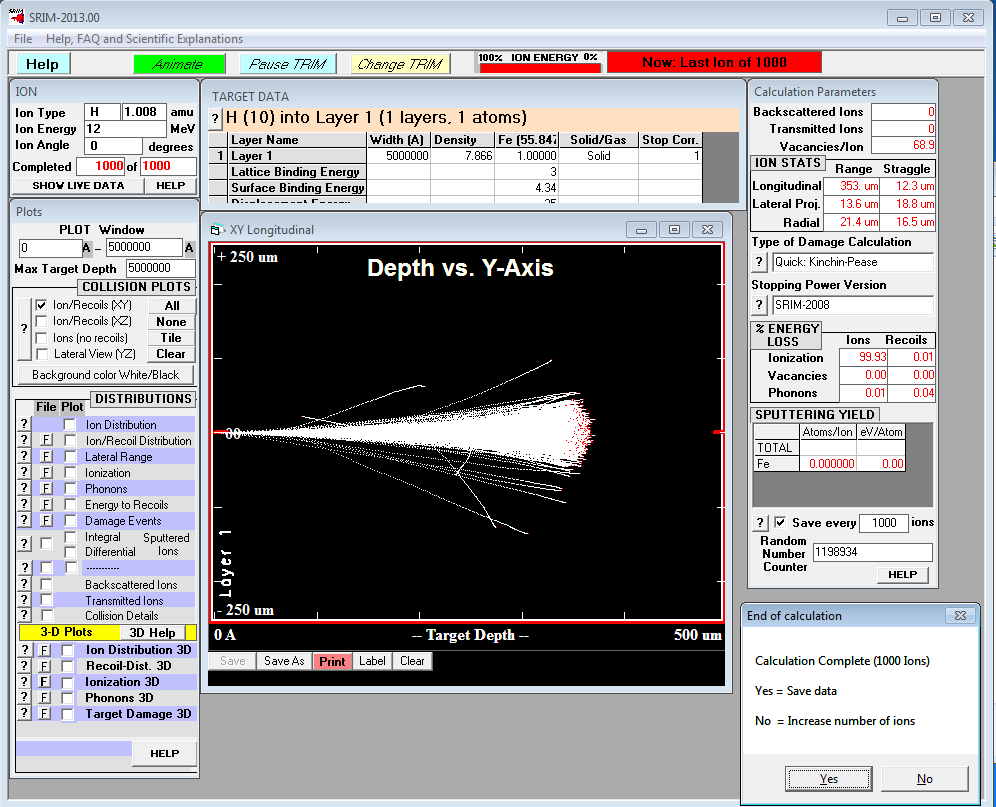
\includegraphics[width=5.0cm]{appendix/srim_data/12MeV.png}
    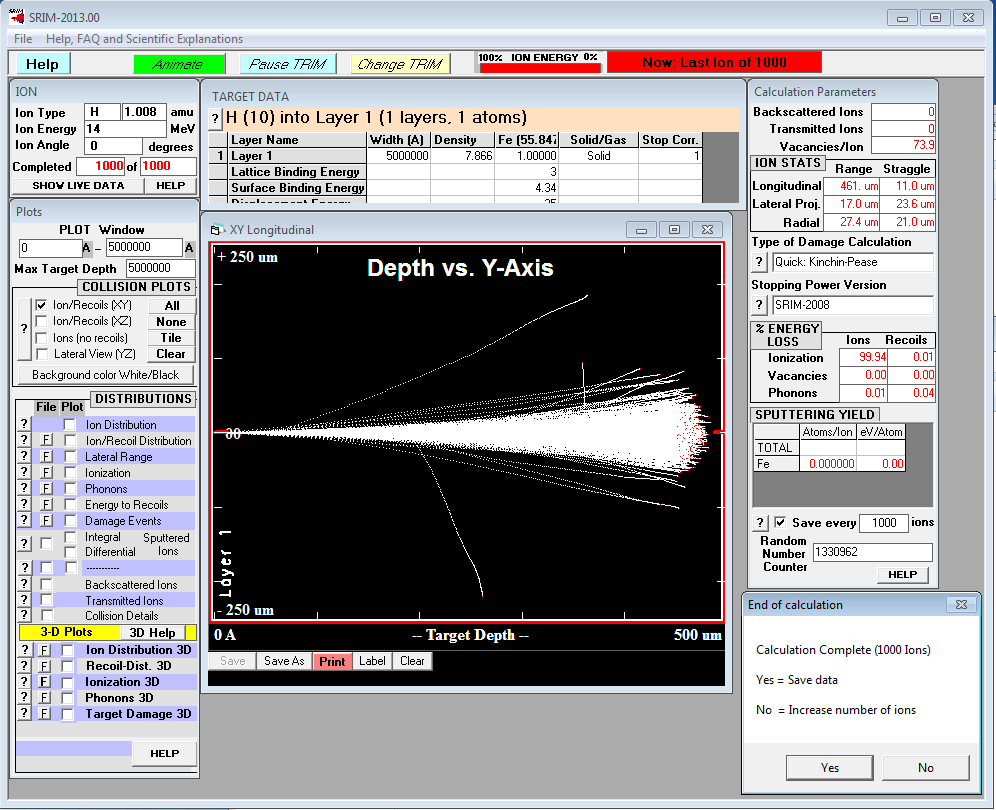
\includegraphics[width=5.0cm]{appendix/srim_data/14MeV.png}
    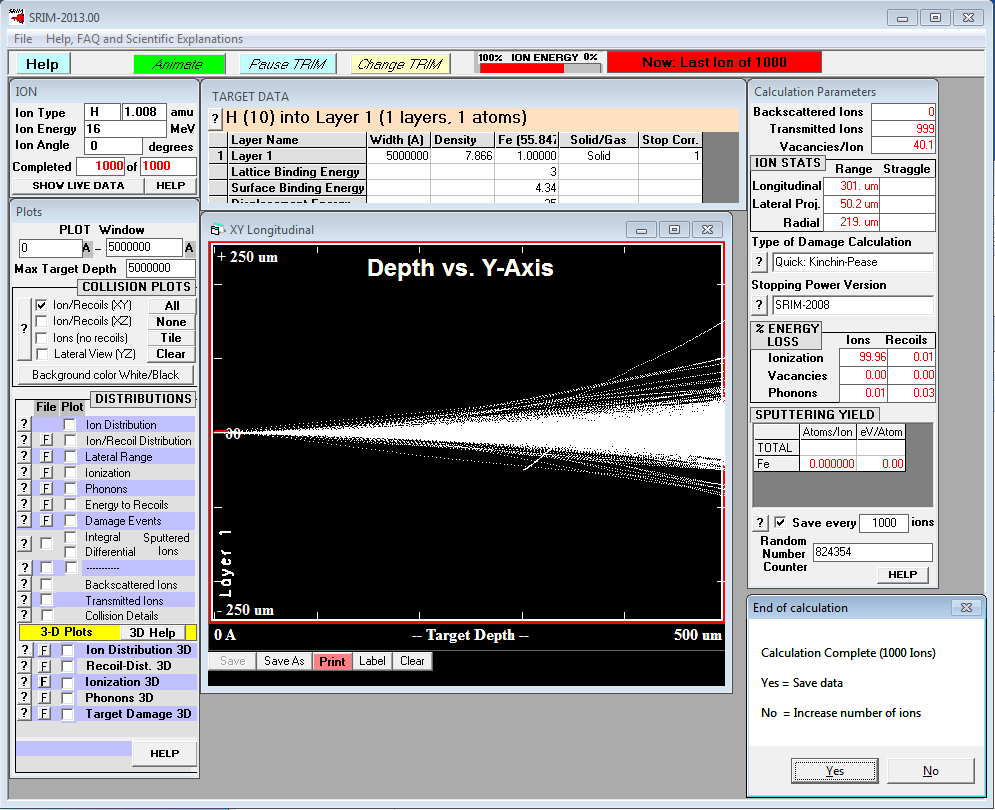
\includegraphics[width=5.0cm]{appendix/srim_data/16MeV.png}
    \caption{SRIM trajectories for 12MeV, 14MeV and 16MeV protons in iron}
    \label{fig:srimiron-12-14-16}
  \end{center}
\end{figure}

\begin{figure}[!htb]
  \begin{center}
    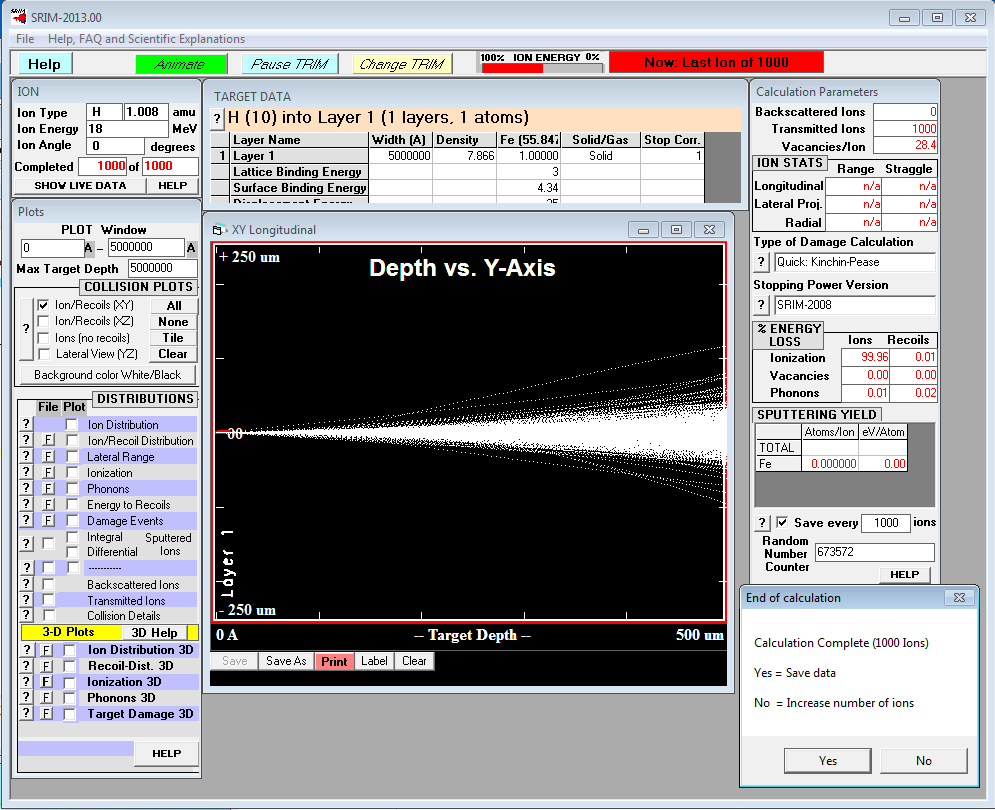
\includegraphics[width=5.0cm]{appendix/srim_data/18MeV.png}
    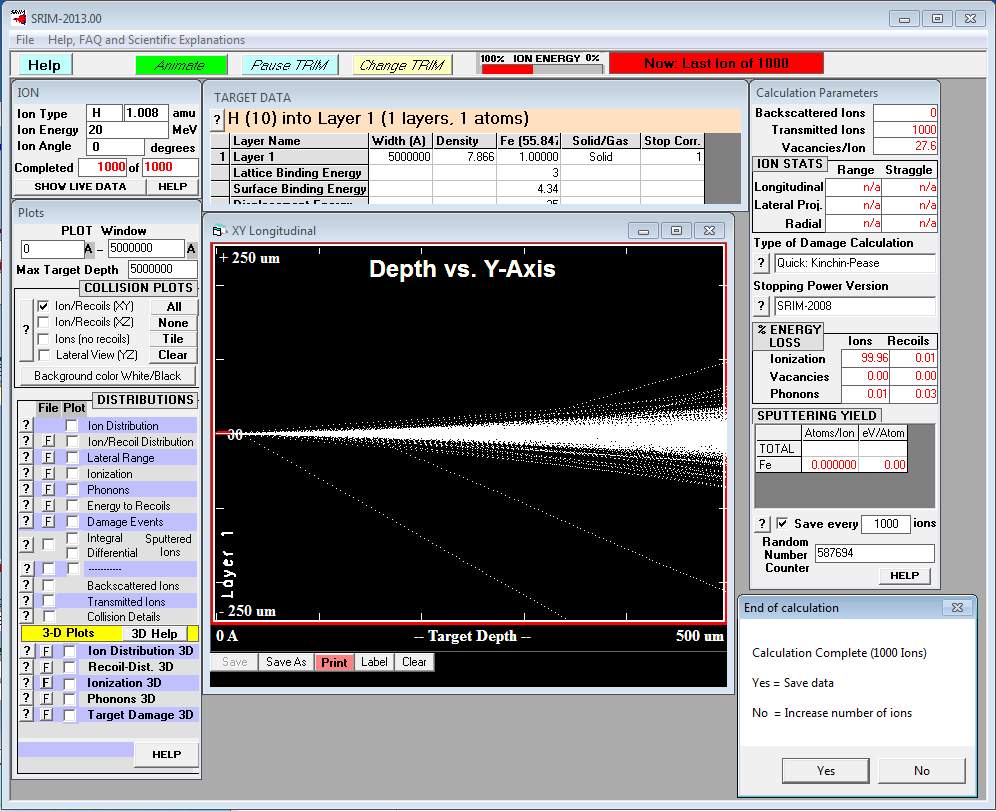
\includegraphics[width=5.0cm]{appendix/srim_data/20MeV.png}
    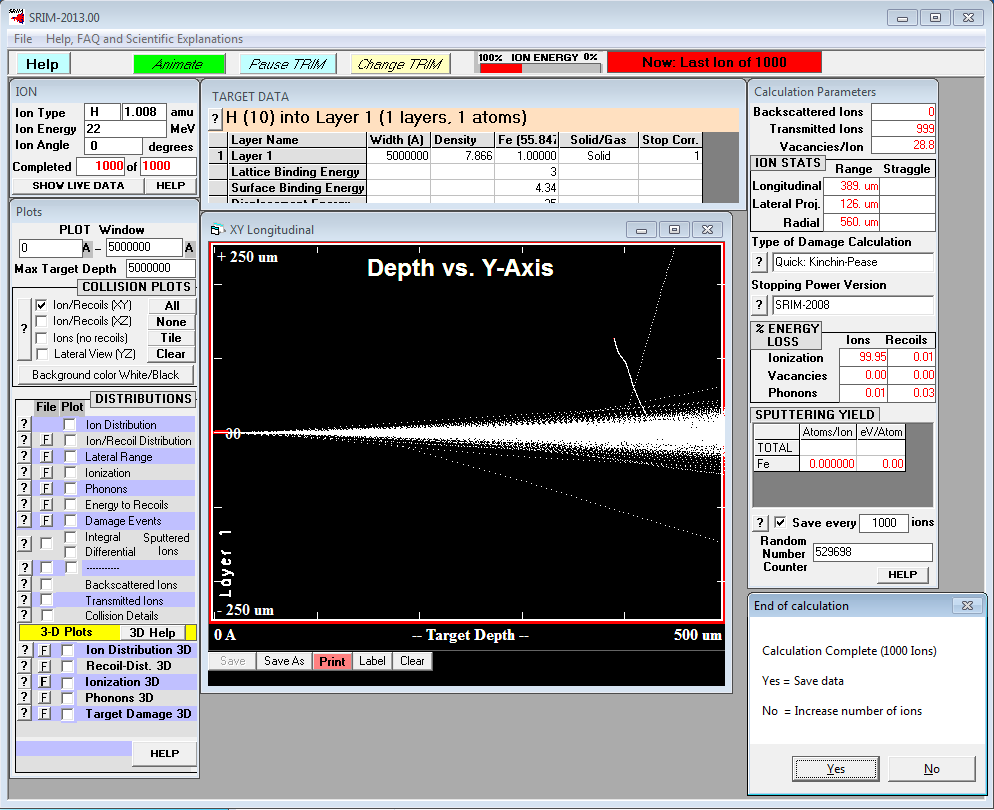
\includegraphics[width=5.0cm]{appendix/srim_data/22MeV.png}
    \caption{SRIM trajectories for 18MeV, 20MeV and 22MeV protons in iron}
    \label{fig:srimiron-18-20-22}
  \end{center}
\end{figure}

\begin{figure}[!htb]
  \begin{center}
    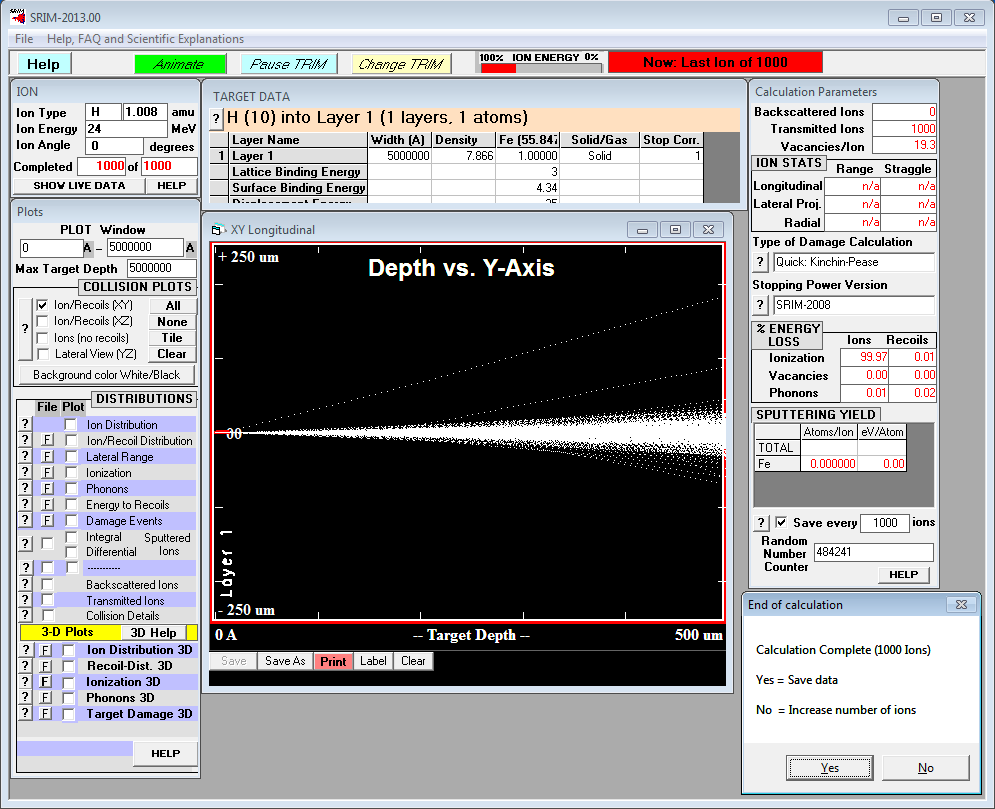
\includegraphics[width=5.0cm]{appendix/srim_data/24MeV.png}
    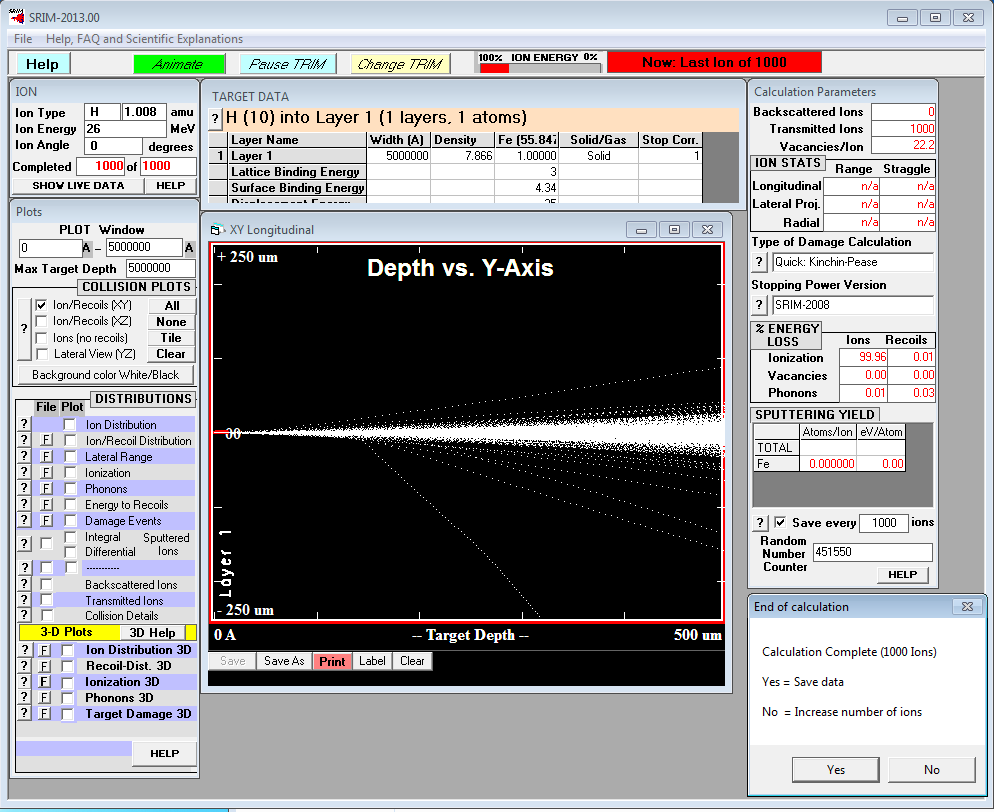
\includegraphics[width=5.0cm]{appendix/srim_data/26MeV.png}
    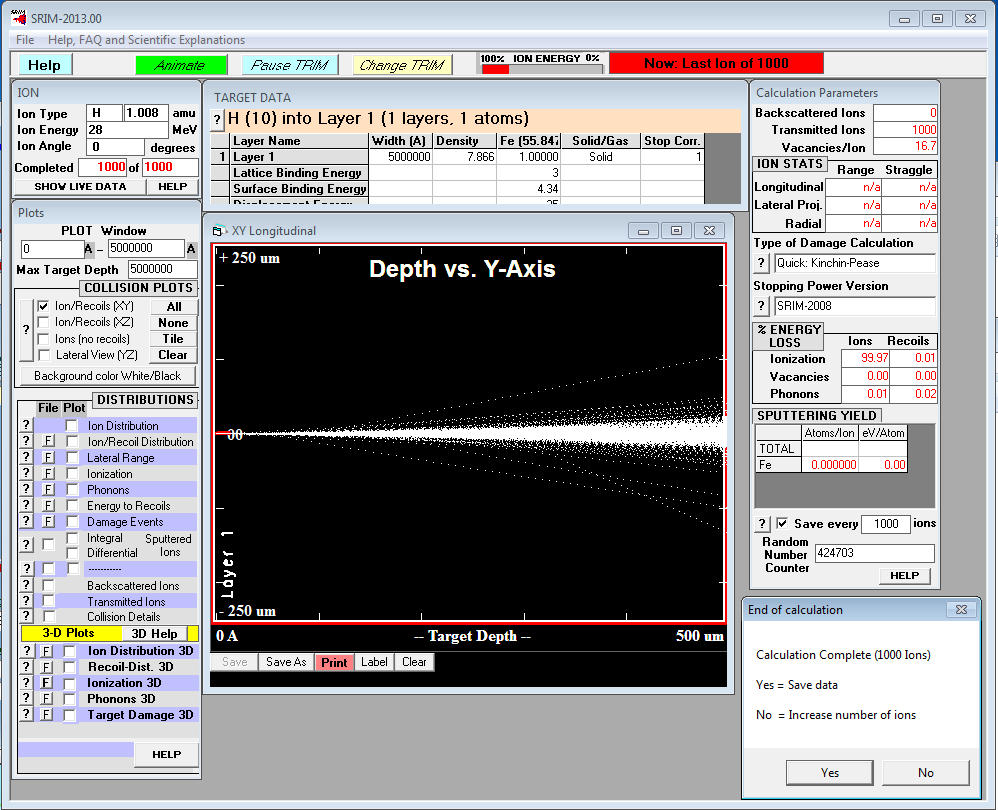
\includegraphics[width=5.0cm]{appendix/srim_data/28MeV.png}
    \caption{SRIM trajectories for 24MeV, 26MeV and 28MeV protons in iron}
    \label{fig:srimiron-24-26-28}
  \end{center}
\end{figure}

\begin{figure}[!htb]
  \begin{center}
    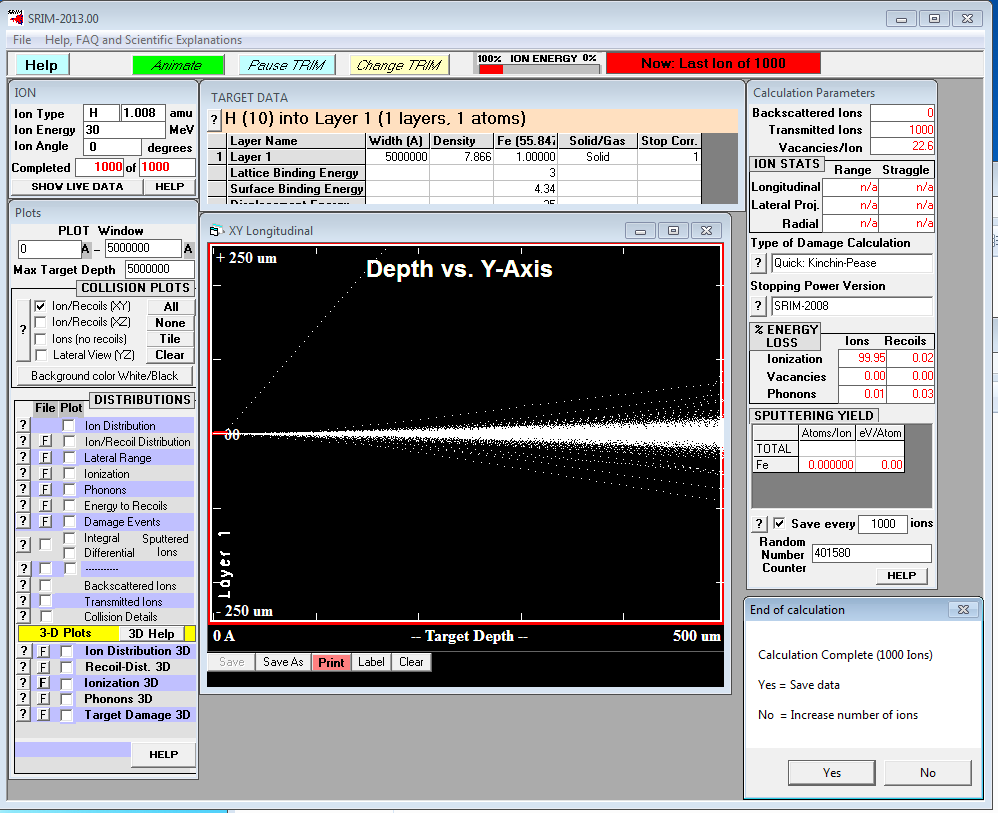
\includegraphics[width=5.0cm]{appendix/srim_data/30MeV.png}
    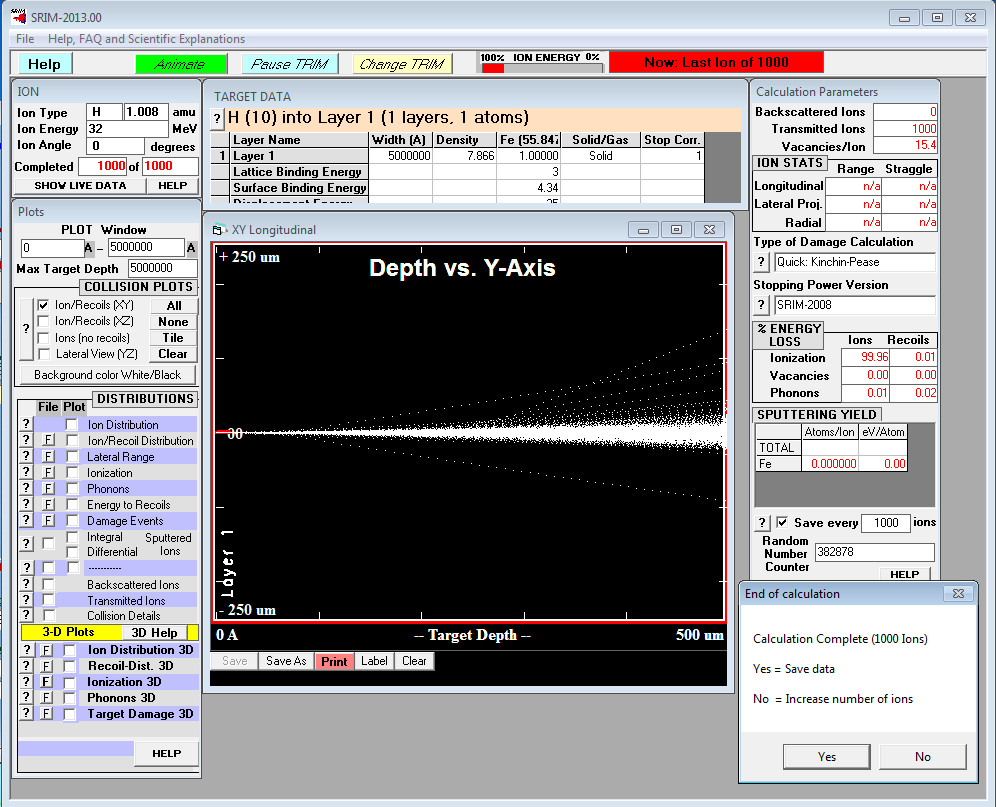
\includegraphics[width=5.0cm]{appendix/srim_data/32MeV.png}
    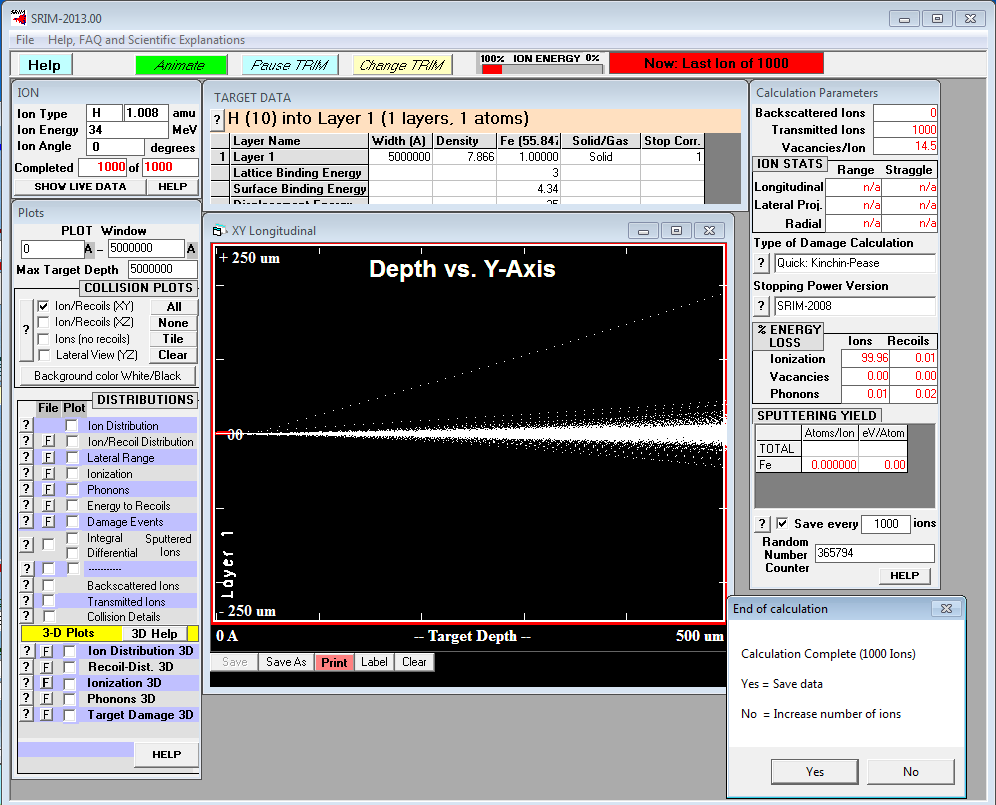
\includegraphics[width=5.0cm]{appendix/srim_data/34MeV.png}
    \caption{SRIM trajectories for 30MeV, 32MeV and 34MeV protons in iron}
    \label{fig:srimiron-30-32-34}
  \end{center}
\end{figure}

\begin{figure}[!htb]
  \begin{center}
    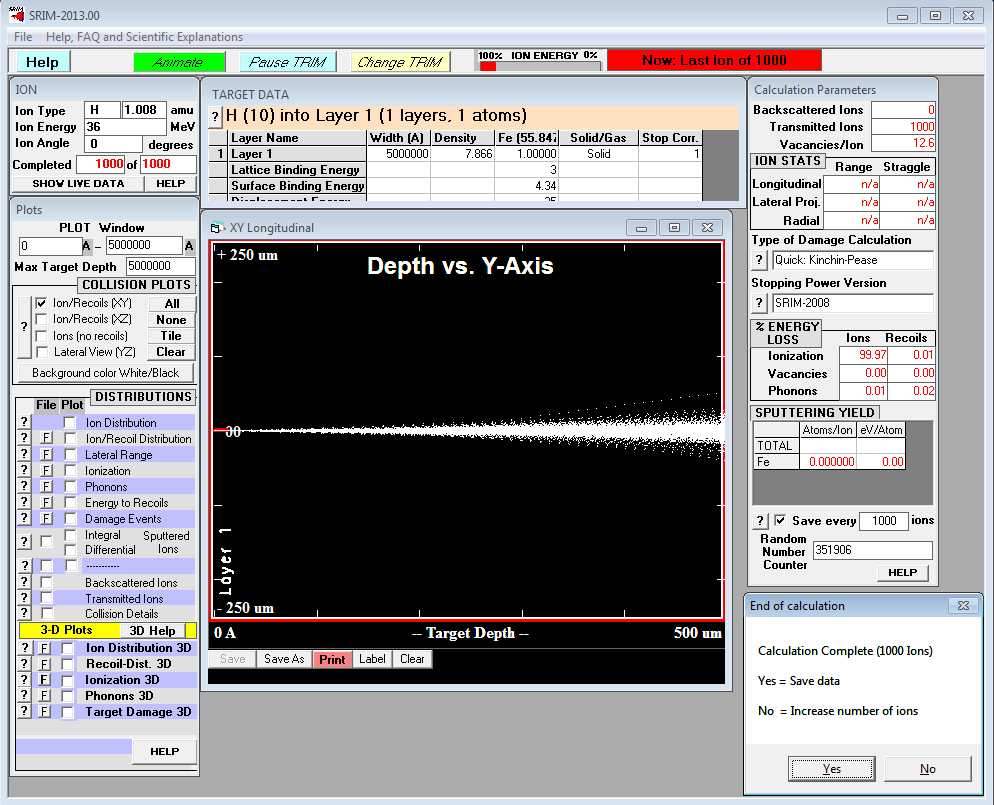
\includegraphics[width=5.0cm]{appendix/srim_data/36MeV.png}
    \caption{SRIM trajectories for 36MeV protons in iron}
    \label{fig:srimiron-36}
  \end{center}
\end{figure}






